% Generated by tools/check_absolute_calibration.py on 2026-11-16 -- do not edit by hand.
% % Generated by tools/check_absolute_calibration.py on 2026-11-16 -- do not edit by hand.
% % Generated by tools/check_absolute_calibration.py on 2026-11-16 -- do not edit by hand.
% % Generated by tools/check_absolute_calibration.py on 2026-11-16 -- do not edit by hand.
% \input{figures/abscal/abscal_mrk817} from docs/ (needs graphicx, booktabs).
\paragraph{Independent check of the absolute calibration (Mrk 817).}
The PyTICS-calibrated comparison stars were compared with photometry that AVA never
uses: SDSS DR16 PSF magnitudes ($u\,g\,r\,i\,z$; $B$, $V$ through the Jordi et al.\ 2006
stellar transformations, themselves good to $\sim$0.02--0.03\,mag) and Pan-STARRS1 DR2
$y$ (Table~\ref{tab:mrk817}, Figs.~\ref{fig:mrk817-stars}--\ref{fig:mrk817-summary}).
Evaluated at the AGN colour ($g-i=0.34$), $u\,g\,r\,i\,z$ agree with SDSS to
$\le0.007$\,mag and $B$, $V$ to $+0.019$--$+0.023$\,mag,
within the transformation uncertainty; the GSPC catalogue itself shows the same $B$, $V$
offset. Individual cameras agree to 0.002--0.010\,mag rms
(Fig.~\ref{fig:mrk817-cameras}), and the per-frame zero points of the \texttt{frame\_qc} path
agree with the ensemble to $\le0.011$\,mag (Fig.~\ref{fig:mrk817-framezp}).
MuSCAT measures the AGN $0.07$--$0.10$\,mag fainter than Sinistro on the same nights (8.9$''$ vs 10.5$''$ aperture: less host light); after the intercal correction the difference is $\le0.002$\,mag (Fig.~\ref{fig:mrk817-muscat}). $Y$ has only 10 epochs and a 0.10\,mag star-to-star scatter against PS1 and is not yet usable. The published fluxes use $f_\nu = 3631\,\mathrm{Jy}\times10^{-0.4\,m_{\rm AB}}$
(checked: ratio 0.99994). The comparison is limited by SDSS's own AB accuracy
($\sim$0.01--0.02\,mag, more in $u$) and tests point sources only; the AGN additionally
depends on the aperture host fraction and on emission lines within the filters.

\begin{table}[htbp]
  \centering\small
  \caption{Mrk 817: calibrated comparison stars minus external photometry (AB, mag).
  Median and robust $\sigma$ over stars; ``at AGN'' is a clipped linear fit in $g-i$ evaluated at
  the AGN colour (bootstrap error); GSPC is the reference catalogue against the same truth;
  camera rms is the scatter of per-camera offsets; ZP is the zero point applied to the AGN.}
  \label{tab:mrk817}
  \begin{tabular}{llrrrrrrr}
  \toprule
  Filter & External & $N$ & Median & $\sigma$ & At AGN & GSPC & Camera rms & ZP \\
  \midrule
  up & SDSS $u$ & 38 & $+0.009$ & 0.029 & $-0.007$\,$\pm$0.006 & $-0.014$ & 0.005 & 22.140 \\
  B & SDSS$\to B$ & 61 & $+0.024$ & 0.039 & $+0.023$\,$\pm$0.006 & $+0.020$ & 0.006 & 23.337 \\
  gp & SDSS $g$ & 64 & $-0.000$ & 0.024 & $-0.002$\,$\pm$0.003 & $+0.007$ & 0.007 & 23.926 \\
  V & SDSS$\to V$ & 61 & $+0.013$ & 0.025 & $+0.019$\,$\pm$0.004 & $+0.027$ & 0.003 & 23.412 \\
  rp & SDSS $r$ & 63 & $+0.000$ & 0.023 & $-0.005$\,$\pm$0.005 & $+0.004$ & 0.002 & 23.753 \\
  ip & SDSS $i$ & 65 & $-0.003$ & 0.017 & $-0.003$\,$\pm$0.003 & $-0.002$ & 0.006 & 23.328 \\
  zs & SDSS $z$ & 25 & $-0.010$ & 0.011 & $-0.001$\,$\pm$0.005 & $-0.006$ & 0.010 & 22.164 \\
  Y & PS1 $y$ & 20 & $-0.017$ & 0.103 & $+0.007$\,$\pm$0.029 & $+0.005$ & -- & 20.110 \\
  \bottomrule
  \end{tabular}
\end{table}

\begin{figure}[htbp]
  \centering
  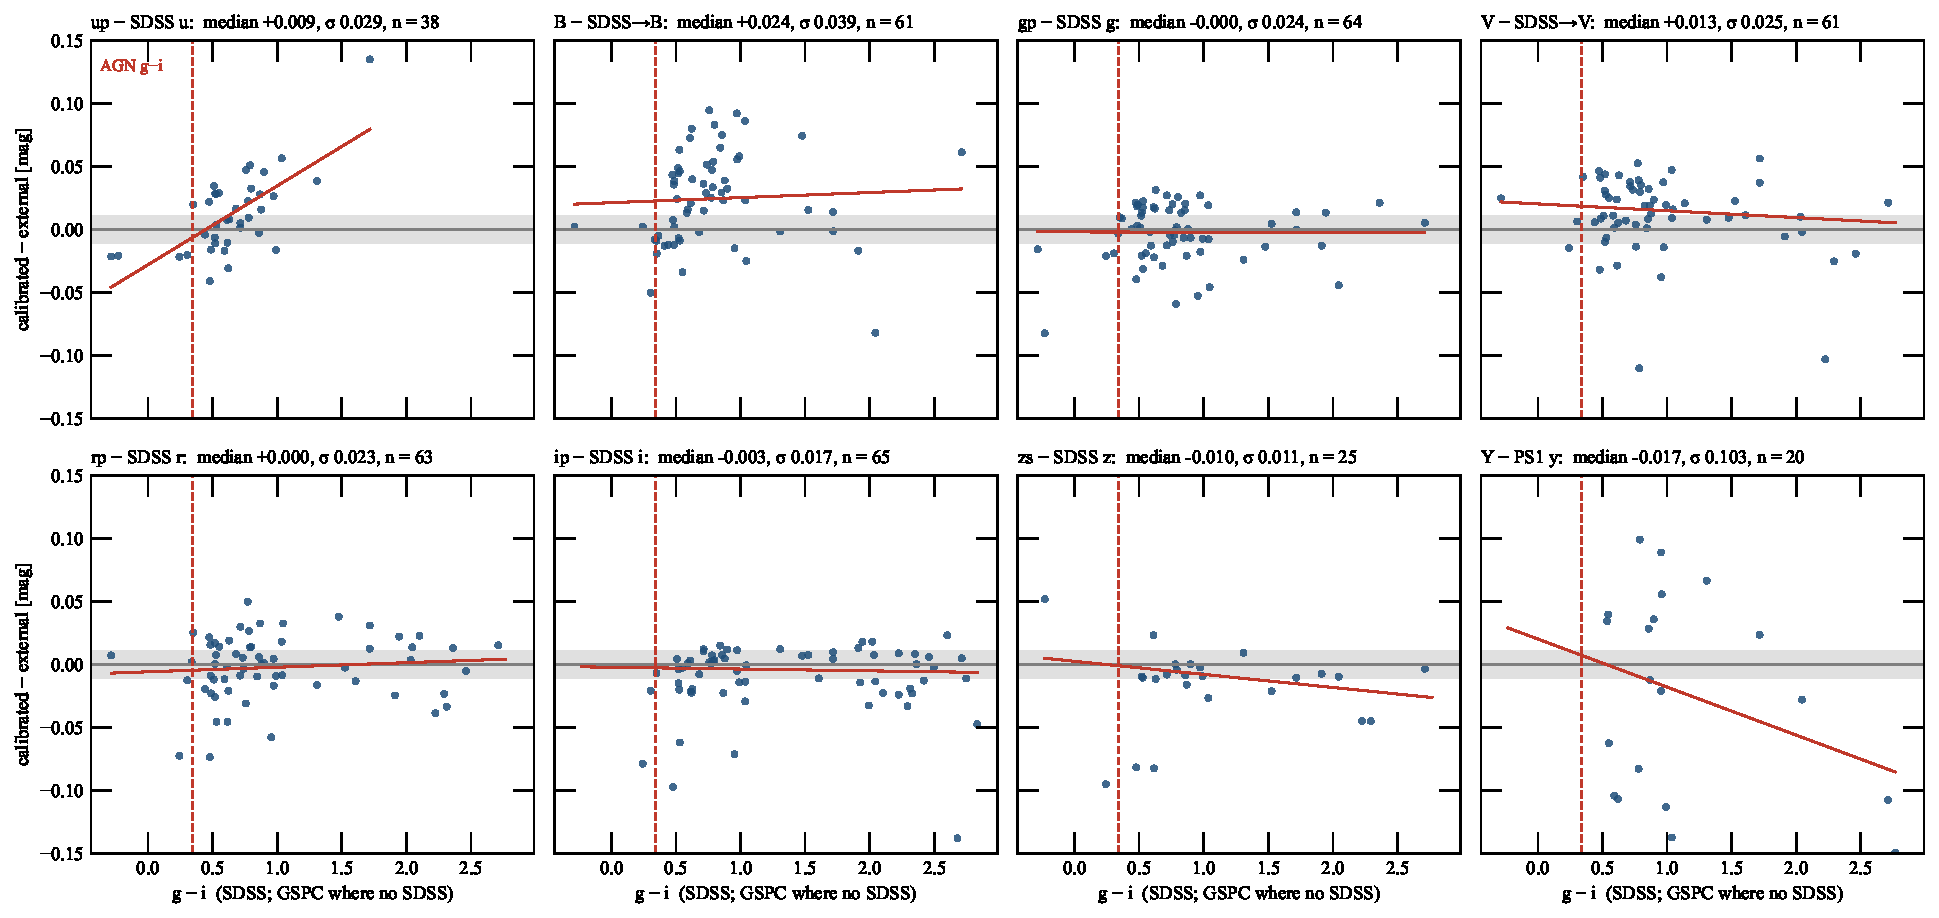
\includegraphics[width=\textwidth]{figures/abscal/abscal_01_stars.pdf}
  \caption{Mrk 817: PyTICS-calibrated comparison stars minus SDSS DR16 ($B$, $V$ via
  Jordi et al.\ 2006) and PS1 DR2 $y$, against $g-i$. Red line: clipped linear fit; dashed:
  AGN colour; grey band: $\pm0.01$\,mag.}
  \label{fig:mrk817-stars}
\end{figure}

\begin{figure}[htbp]
  \centering
  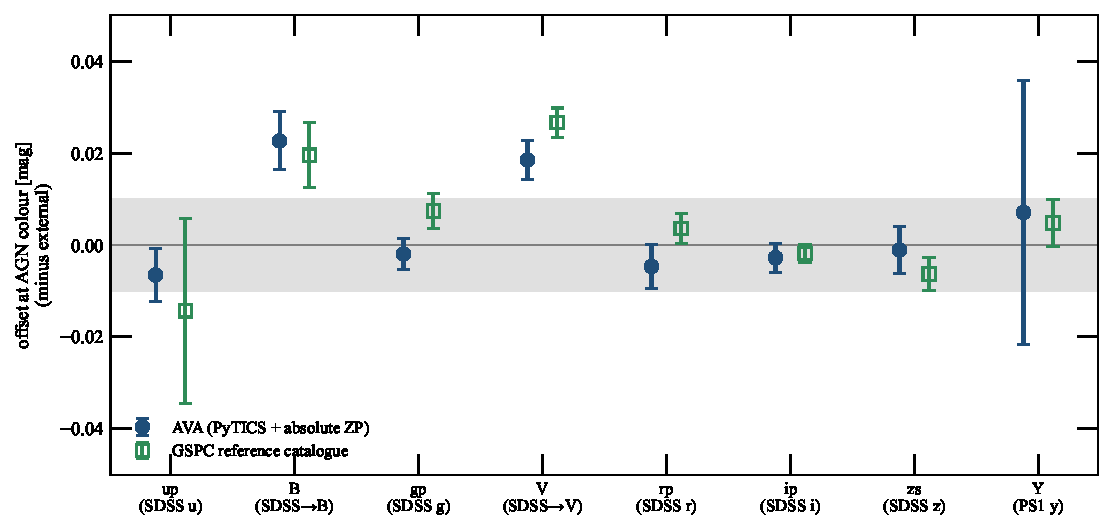
\includegraphics[width=0.75\textwidth]{figures/abscal/abscal_02_summary.pdf}
  \caption{Mrk 817: offset from the external photometry at the AGN colour, for the AVA
  calibration (filled) and for the GSPC reference catalogue (open).}
  \label{fig:mrk817-summary}
\end{figure}

\begin{figure}[htbp]
  \centering
  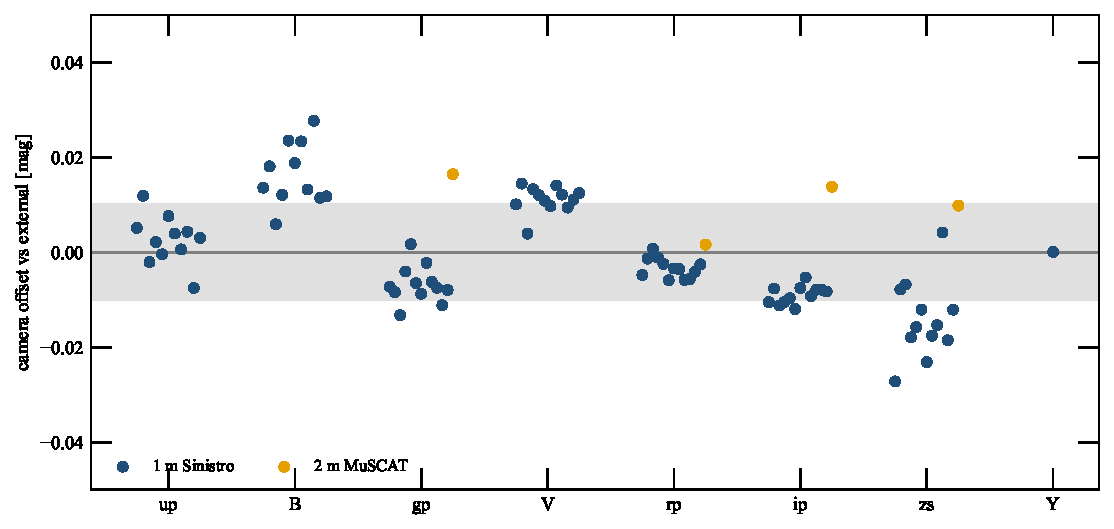
\includegraphics[width=0.75\textwidth]{figures/abscal/abscal_03_cameras.pdf}
  \caption{Mrk 817: per-camera offset from the external photometry (median over stars of
  each star's median calibrated magnitude in that camera).}
  \label{fig:mrk817-cameras}
\end{figure}

\begin{figure}[htbp]
  \centering
  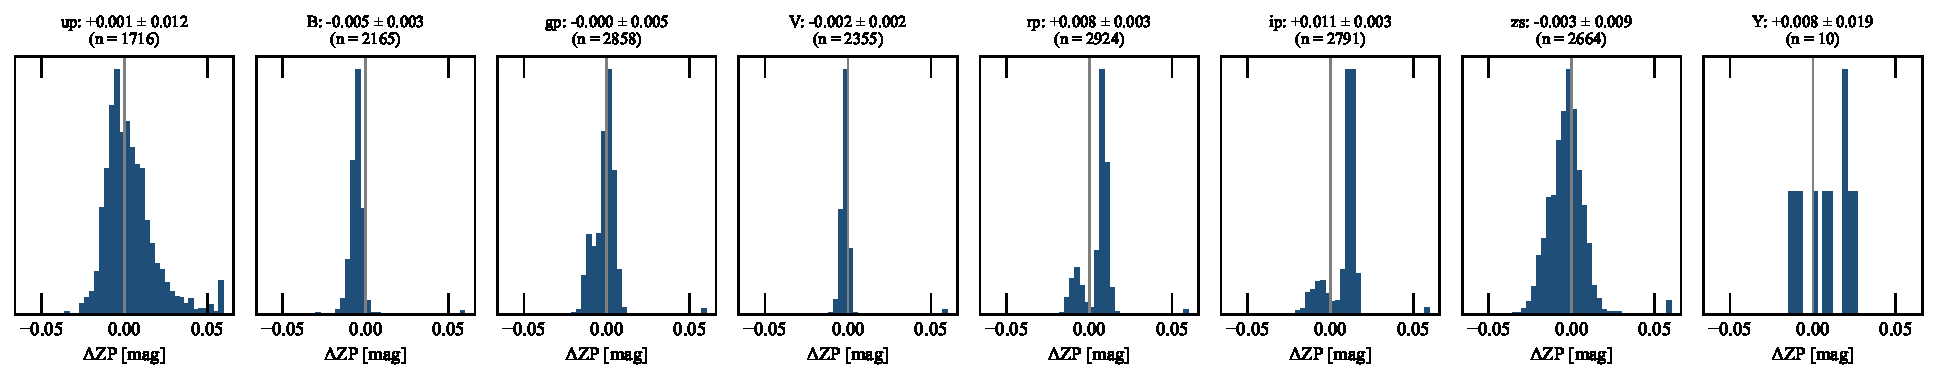
\includegraphics[width=\textwidth]{figures/abscal/abscal_04_frame_zp.pdf}
  \caption{Mrk 817: per-frame zero point from \texttt{frame\_qc} minus the ensemble
  zero point of the same frame (median $\pm$ robust $\sigma$). The secondary peak in $r$ and
  $i$ is MuSCAT (few ZP stars in its small field); Sinistro frames sit at a constant offset.
  The AGN light curve uses the ensemble zero point only.}
  \label{fig:mrk817-framezp}
\end{figure}

\begin{figure}[htbp]
  \centering
  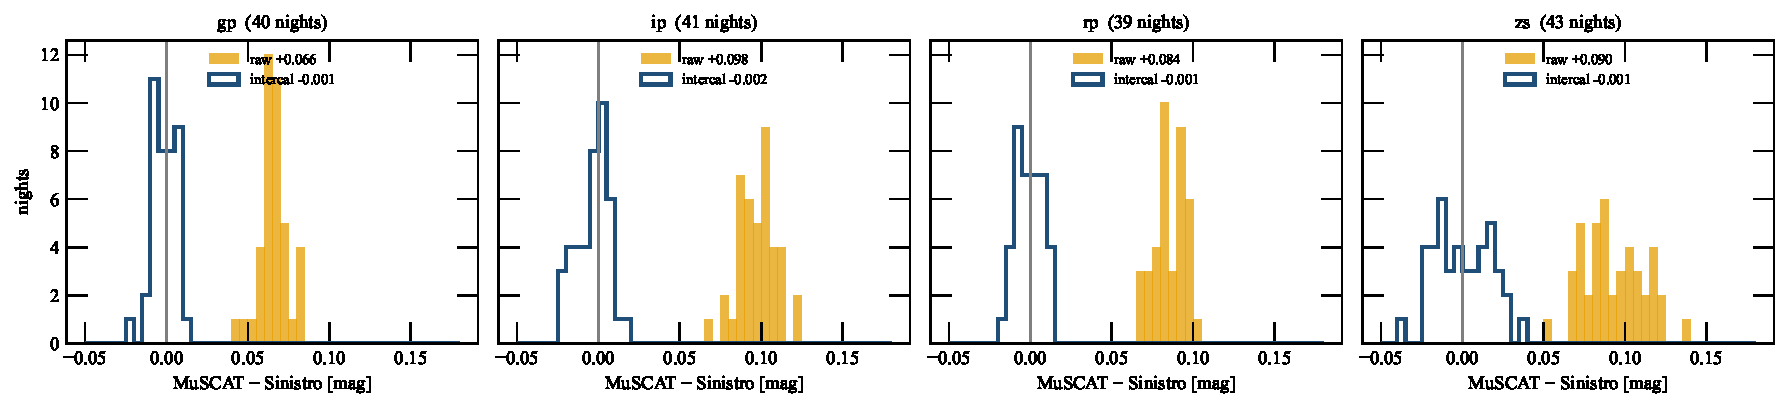
\includegraphics[width=\textwidth]{figures/abscal/abscal_05_muscat.pdf}
  \caption{Mrk 817: AGN, MuSCAT minus Sinistro on the same night, before (filled) and
  after (open) the additive intercal correction.}
  \label{fig:mrk817-muscat}
\end{figure}
 from docs/ (needs graphicx, booktabs).
\paragraph{Independent check of the absolute calibration (Mrk 817).}
The PyTICS-calibrated comparison stars were compared with photometry that AVA never
uses: SDSS DR16 PSF magnitudes ($u\,g\,r\,i\,z$; $B$, $V$ through the Jordi et al.\ 2006
stellar transformations, themselves good to $\sim$0.02--0.03\,mag) and Pan-STARRS1 DR2
$y$ (Table~\ref{tab:mrk817}, Figs.~\ref{fig:mrk817-stars}--\ref{fig:mrk817-summary}).
Evaluated at the AGN colour ($g-i=0.34$), $u\,g\,r\,i\,z$ agree with SDSS to
$\le0.007$\,mag and $B$, $V$ to $+0.019$--$+0.023$\,mag,
within the transformation uncertainty; the GSPC catalogue itself shows the same $B$, $V$
offset. Individual cameras agree to 0.002--0.010\,mag rms
(Fig.~\ref{fig:mrk817-cameras}), and the per-frame zero points of the \texttt{frame\_qc} path
agree with the ensemble to $\le0.011$\,mag (Fig.~\ref{fig:mrk817-framezp}).
MuSCAT measures the AGN $0.07$--$0.10$\,mag fainter than Sinistro on the same nights (8.9$''$ vs 10.5$''$ aperture: less host light); after the intercal correction the difference is $\le0.002$\,mag (Fig.~\ref{fig:mrk817-muscat}). $Y$ has only 10 epochs and a 0.10\,mag star-to-star scatter against PS1 and is not yet usable. The published fluxes use $f_\nu = 3631\,\mathrm{Jy}\times10^{-0.4\,m_{\rm AB}}$
(checked: ratio 0.99994). The comparison is limited by SDSS's own AB accuracy
($\sim$0.01--0.02\,mag, more in $u$) and tests point sources only; the AGN additionally
depends on the aperture host fraction and on emission lines within the filters.

\begin{table}[htbp]
  \centering\small
  \caption{Mrk 817: calibrated comparison stars minus external photometry (AB, mag).
  Median and robust $\sigma$ over stars; ``at AGN'' is a clipped linear fit in $g-i$ evaluated at
  the AGN colour (bootstrap error); GSPC is the reference catalogue against the same truth;
  camera rms is the scatter of per-camera offsets; ZP is the zero point applied to the AGN.}
  \label{tab:mrk817}
  \begin{tabular}{llrrrrrrr}
  \toprule
  Filter & External & $N$ & Median & $\sigma$ & At AGN & GSPC & Camera rms & ZP \\
  \midrule
  up & SDSS $u$ & 38 & $+0.009$ & 0.029 & $-0.007$\,$\pm$0.006 & $-0.014$ & 0.005 & 22.140 \\
  B & SDSS$\to B$ & 61 & $+0.024$ & 0.039 & $+0.023$\,$\pm$0.006 & $+0.020$ & 0.006 & 23.337 \\
  gp & SDSS $g$ & 64 & $-0.000$ & 0.024 & $-0.002$\,$\pm$0.003 & $+0.007$ & 0.007 & 23.926 \\
  V & SDSS$\to V$ & 61 & $+0.013$ & 0.025 & $+0.019$\,$\pm$0.004 & $+0.027$ & 0.003 & 23.412 \\
  rp & SDSS $r$ & 63 & $+0.000$ & 0.023 & $-0.005$\,$\pm$0.005 & $+0.004$ & 0.002 & 23.753 \\
  ip & SDSS $i$ & 65 & $-0.003$ & 0.017 & $-0.003$\,$\pm$0.003 & $-0.002$ & 0.006 & 23.328 \\
  zs & SDSS $z$ & 25 & $-0.010$ & 0.011 & $-0.001$\,$\pm$0.005 & $-0.006$ & 0.010 & 22.164 \\
  Y & PS1 $y$ & 20 & $-0.017$ & 0.103 & $+0.007$\,$\pm$0.029 & $+0.005$ & -- & 20.110 \\
  \bottomrule
  \end{tabular}
\end{table}

\begin{figure}[htbp]
  \centering
  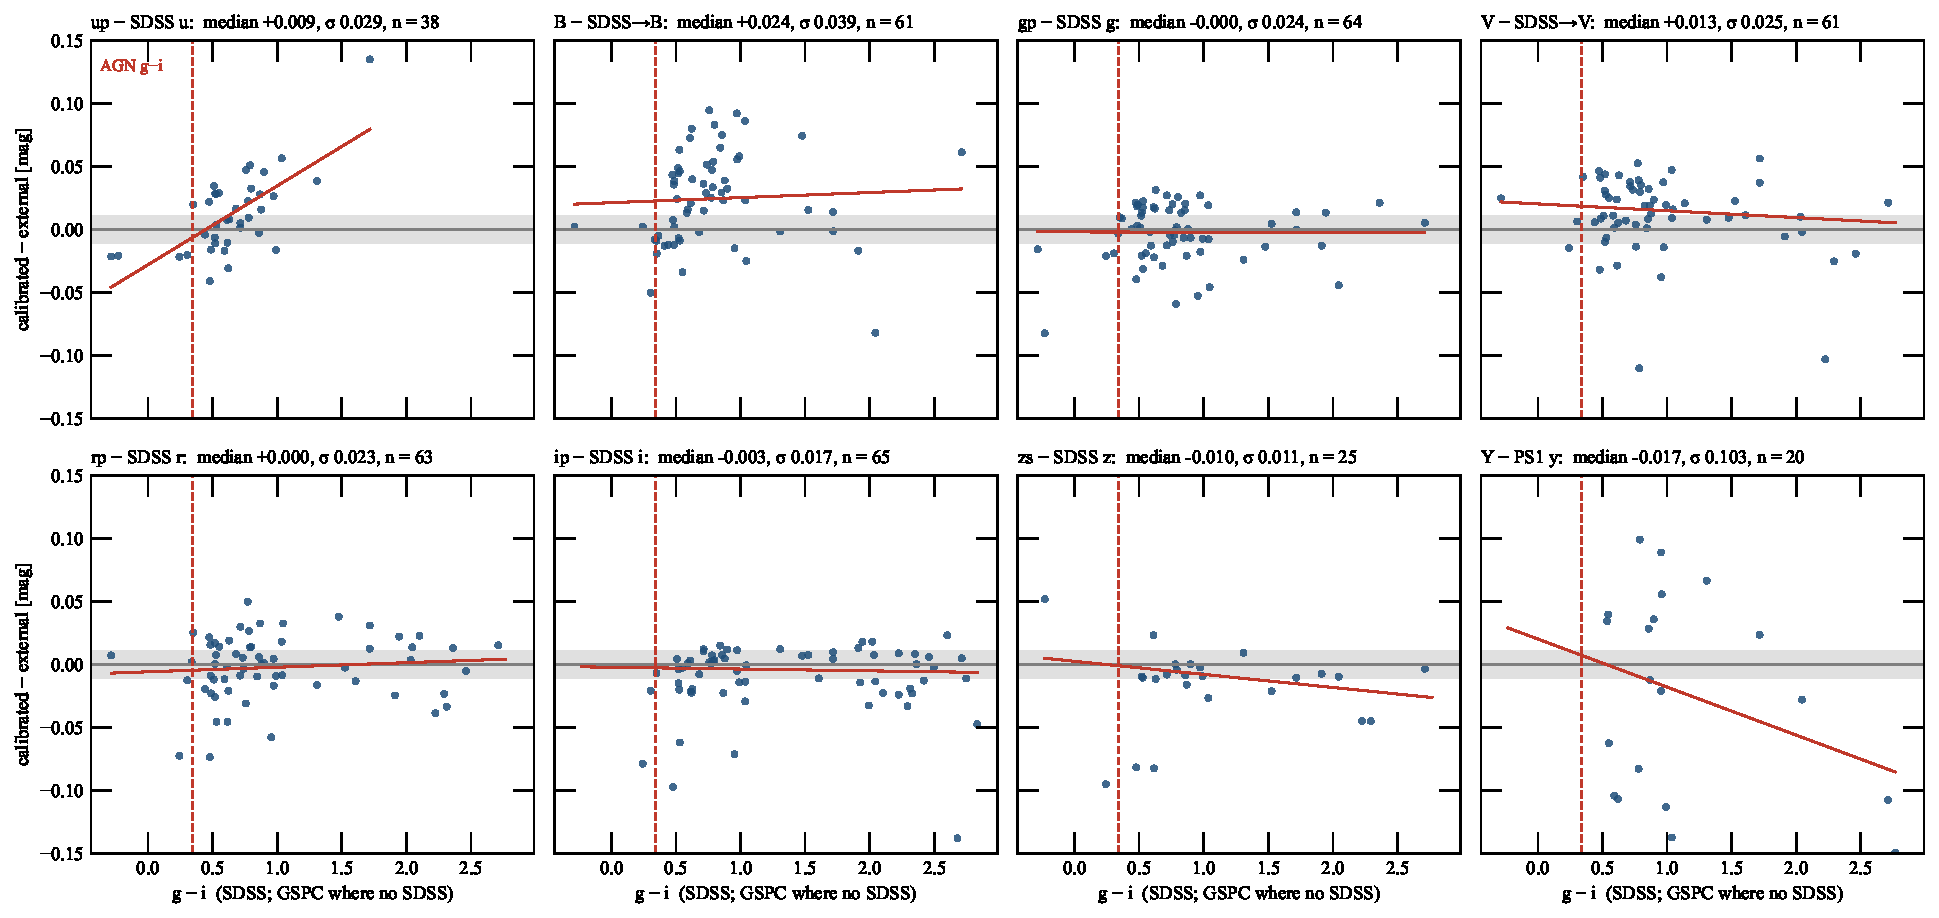
\includegraphics[width=\textwidth]{figures/abscal/abscal_01_stars.pdf}
  \caption{Mrk 817: PyTICS-calibrated comparison stars minus SDSS DR16 ($B$, $V$ via
  Jordi et al.\ 2006) and PS1 DR2 $y$, against $g-i$. Red line: clipped linear fit; dashed:
  AGN colour; grey band: $\pm0.01$\,mag.}
  \label{fig:mrk817-stars}
\end{figure}

\begin{figure}[htbp]
  \centering
  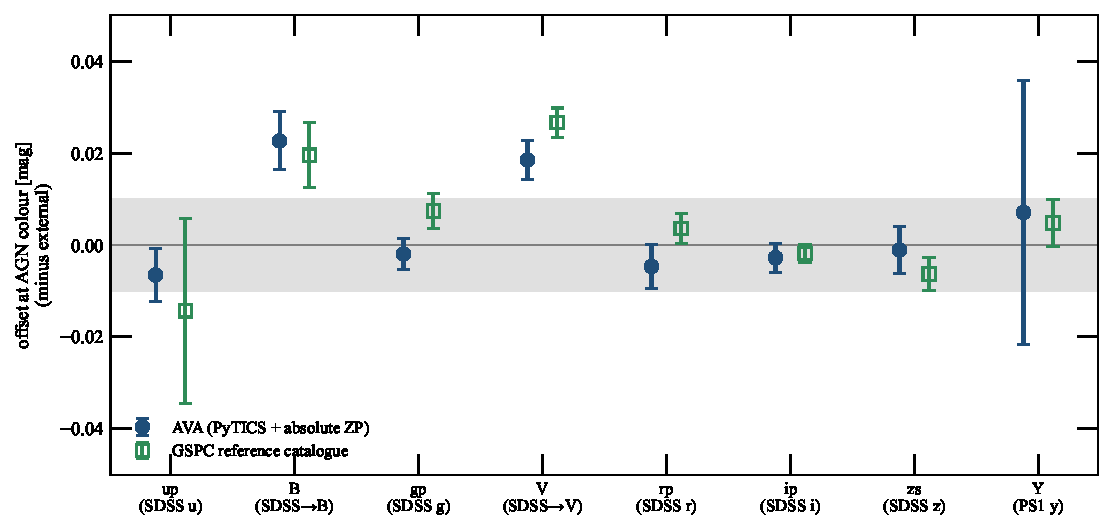
\includegraphics[width=0.75\textwidth]{figures/abscal/abscal_02_summary.pdf}
  \caption{Mrk 817: offset from the external photometry at the AGN colour, for the AVA
  calibration (filled) and for the GSPC reference catalogue (open).}
  \label{fig:mrk817-summary}
\end{figure}

\begin{figure}[htbp]
  \centering
  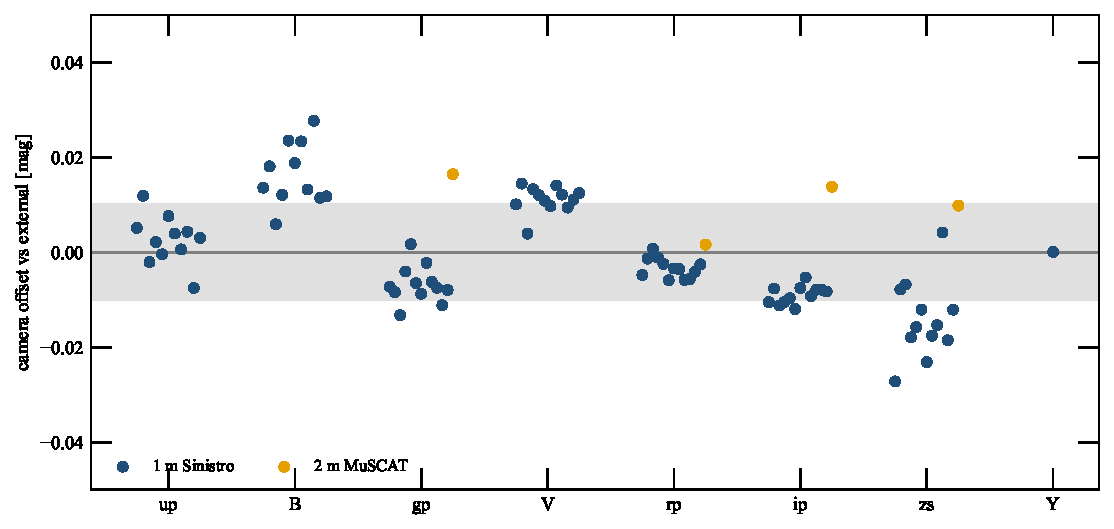
\includegraphics[width=0.75\textwidth]{figures/abscal/abscal_03_cameras.pdf}
  \caption{Mrk 817: per-camera offset from the external photometry (median over stars of
  each star's median calibrated magnitude in that camera).}
  \label{fig:mrk817-cameras}
\end{figure}

\begin{figure}[htbp]
  \centering
  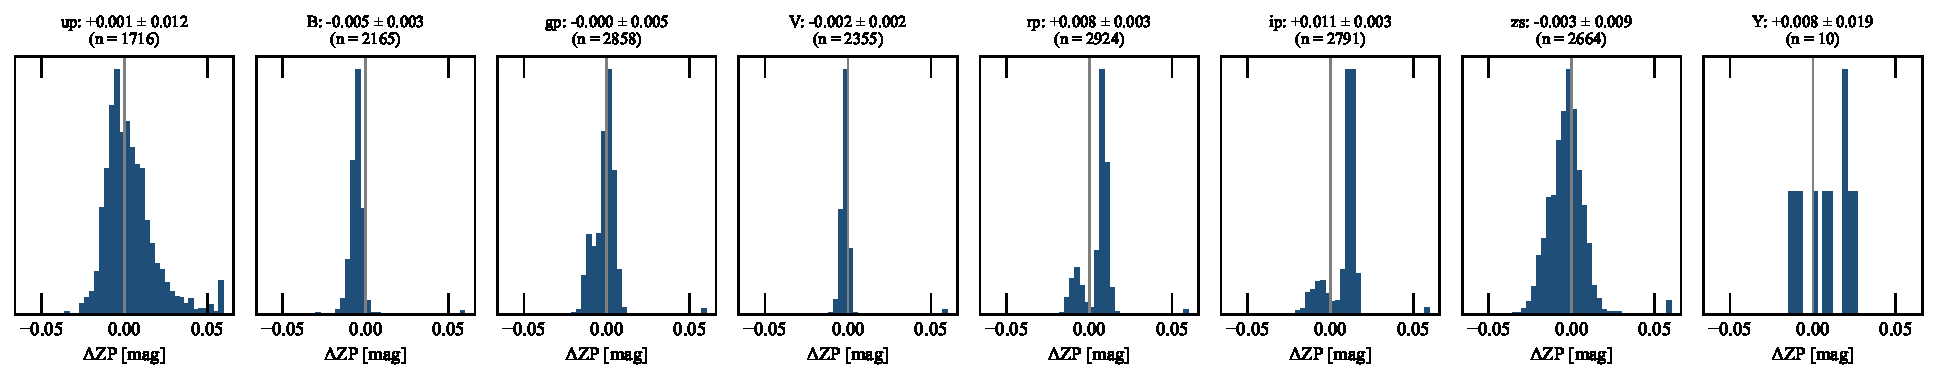
\includegraphics[width=\textwidth]{figures/abscal/abscal_04_frame_zp.pdf}
  \caption{Mrk 817: per-frame zero point from \texttt{frame\_qc} minus the ensemble
  zero point of the same frame (median $\pm$ robust $\sigma$). The secondary peak in $r$ and
  $i$ is MuSCAT (few ZP stars in its small field); Sinistro frames sit at a constant offset.
  The AGN light curve uses the ensemble zero point only.}
  \label{fig:mrk817-framezp}
\end{figure}

\begin{figure}[htbp]
  \centering
  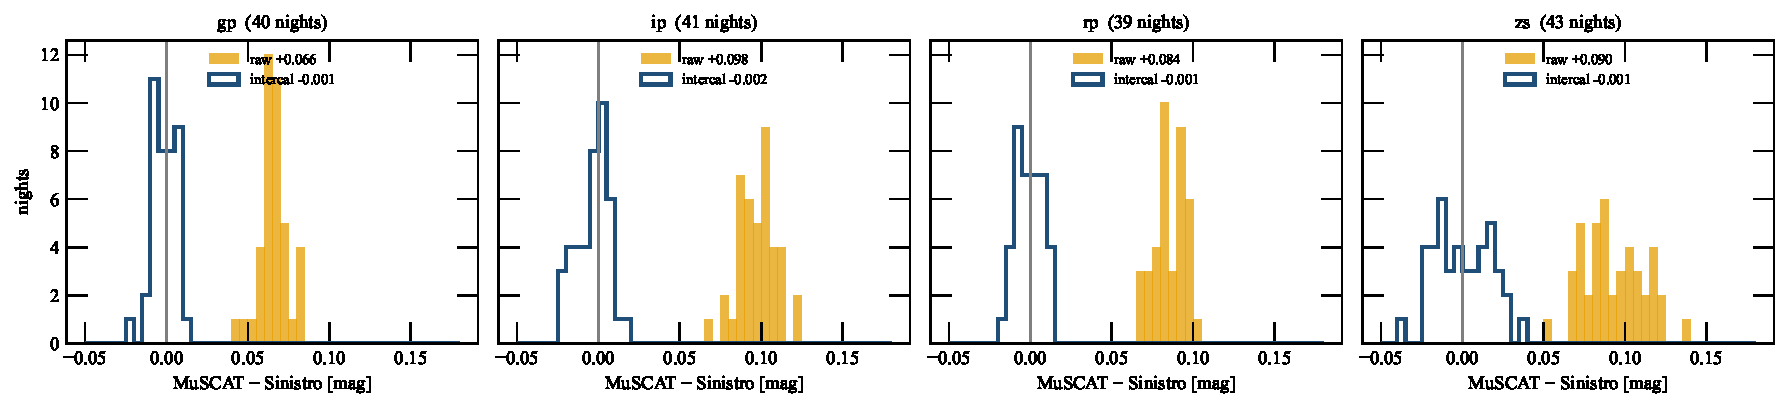
\includegraphics[width=\textwidth]{figures/abscal/abscal_05_muscat.pdf}
  \caption{Mrk 817: AGN, MuSCAT minus Sinistro on the same night, before (filled) and
  after (open) the additive intercal correction.}
  \label{fig:mrk817-muscat}
\end{figure}
 from docs/ (needs graphicx, booktabs).
\paragraph{Independent check of the absolute calibration (Mrk 817).}
The PyTICS-calibrated comparison stars were compared with photometry that AVA never
uses: SDSS DR16 PSF magnitudes ($u\,g\,r\,i\,z$; $B$, $V$ through the Jordi et al.\ 2006
stellar transformations, themselves good to $\sim$0.02--0.03\,mag) and Pan-STARRS1 DR2
$y$ (Table~\ref{tab:mrk817}, Figs.~\ref{fig:mrk817-stars}--\ref{fig:mrk817-summary}).
Evaluated at the AGN colour ($g-i=0.34$), $u\,g\,r\,i\,z$ agree with SDSS to
$\le0.007$\,mag and $B$, $V$ to $+0.019$--$+0.023$\,mag,
within the transformation uncertainty; the GSPC catalogue itself shows the same $B$, $V$
offset. Individual cameras agree to 0.002--0.010\,mag rms
(Fig.~\ref{fig:mrk817-cameras}), and the per-frame zero points of the \texttt{frame\_qc} path
agree with the ensemble to $\le0.011$\,mag (Fig.~\ref{fig:mrk817-framezp}).
MuSCAT measures the AGN $0.07$--$0.10$\,mag fainter than Sinistro on the same nights (8.9$''$ vs 10.5$''$ aperture: less host light); after the intercal correction the difference is $\le0.002$\,mag (Fig.~\ref{fig:mrk817-muscat}). $Y$ has only 10 epochs and a 0.10\,mag star-to-star scatter against PS1 and is not yet usable. The published fluxes use $f_\nu = 3631\,\mathrm{Jy}\times10^{-0.4\,m_{\rm AB}}$
(checked: ratio 0.99994). The comparison is limited by SDSS's own AB accuracy
($\sim$0.01--0.02\,mag, more in $u$) and tests point sources only; the AGN additionally
depends on the aperture host fraction and on emission lines within the filters.

\begin{table}[htbp]
  \centering\small
  \caption{Mrk 817: calibrated comparison stars minus external photometry (AB, mag).
  Median and robust $\sigma$ over stars; ``at AGN'' is a clipped linear fit in $g-i$ evaluated at
  the AGN colour (bootstrap error); GSPC is the reference catalogue against the same truth;
  camera rms is the scatter of per-camera offsets; ZP is the zero point applied to the AGN.}
  \label{tab:mrk817}
  \begin{tabular}{llrrrrrrr}
  \toprule
  Filter & External & $N$ & Median & $\sigma$ & At AGN & GSPC & Camera rms & ZP \\
  \midrule
  up & SDSS $u$ & 38 & $+0.009$ & 0.029 & $-0.007$\,$\pm$0.006 & $-0.014$ & 0.005 & 22.140 \\
  B & SDSS$\to B$ & 61 & $+0.024$ & 0.039 & $+0.023$\,$\pm$0.006 & $+0.020$ & 0.006 & 23.337 \\
  gp & SDSS $g$ & 64 & $-0.000$ & 0.024 & $-0.002$\,$\pm$0.003 & $+0.007$ & 0.007 & 23.926 \\
  V & SDSS$\to V$ & 61 & $+0.013$ & 0.025 & $+0.019$\,$\pm$0.004 & $+0.027$ & 0.003 & 23.412 \\
  rp & SDSS $r$ & 63 & $+0.000$ & 0.023 & $-0.005$\,$\pm$0.005 & $+0.004$ & 0.002 & 23.753 \\
  ip & SDSS $i$ & 65 & $-0.003$ & 0.017 & $-0.003$\,$\pm$0.003 & $-0.002$ & 0.006 & 23.328 \\
  zs & SDSS $z$ & 25 & $-0.010$ & 0.011 & $-0.001$\,$\pm$0.005 & $-0.006$ & 0.010 & 22.164 \\
  Y & PS1 $y$ & 20 & $-0.017$ & 0.103 & $+0.007$\,$\pm$0.029 & $+0.005$ & -- & 20.110 \\
  \bottomrule
  \end{tabular}
\end{table}

\begin{figure}[htbp]
  \centering
  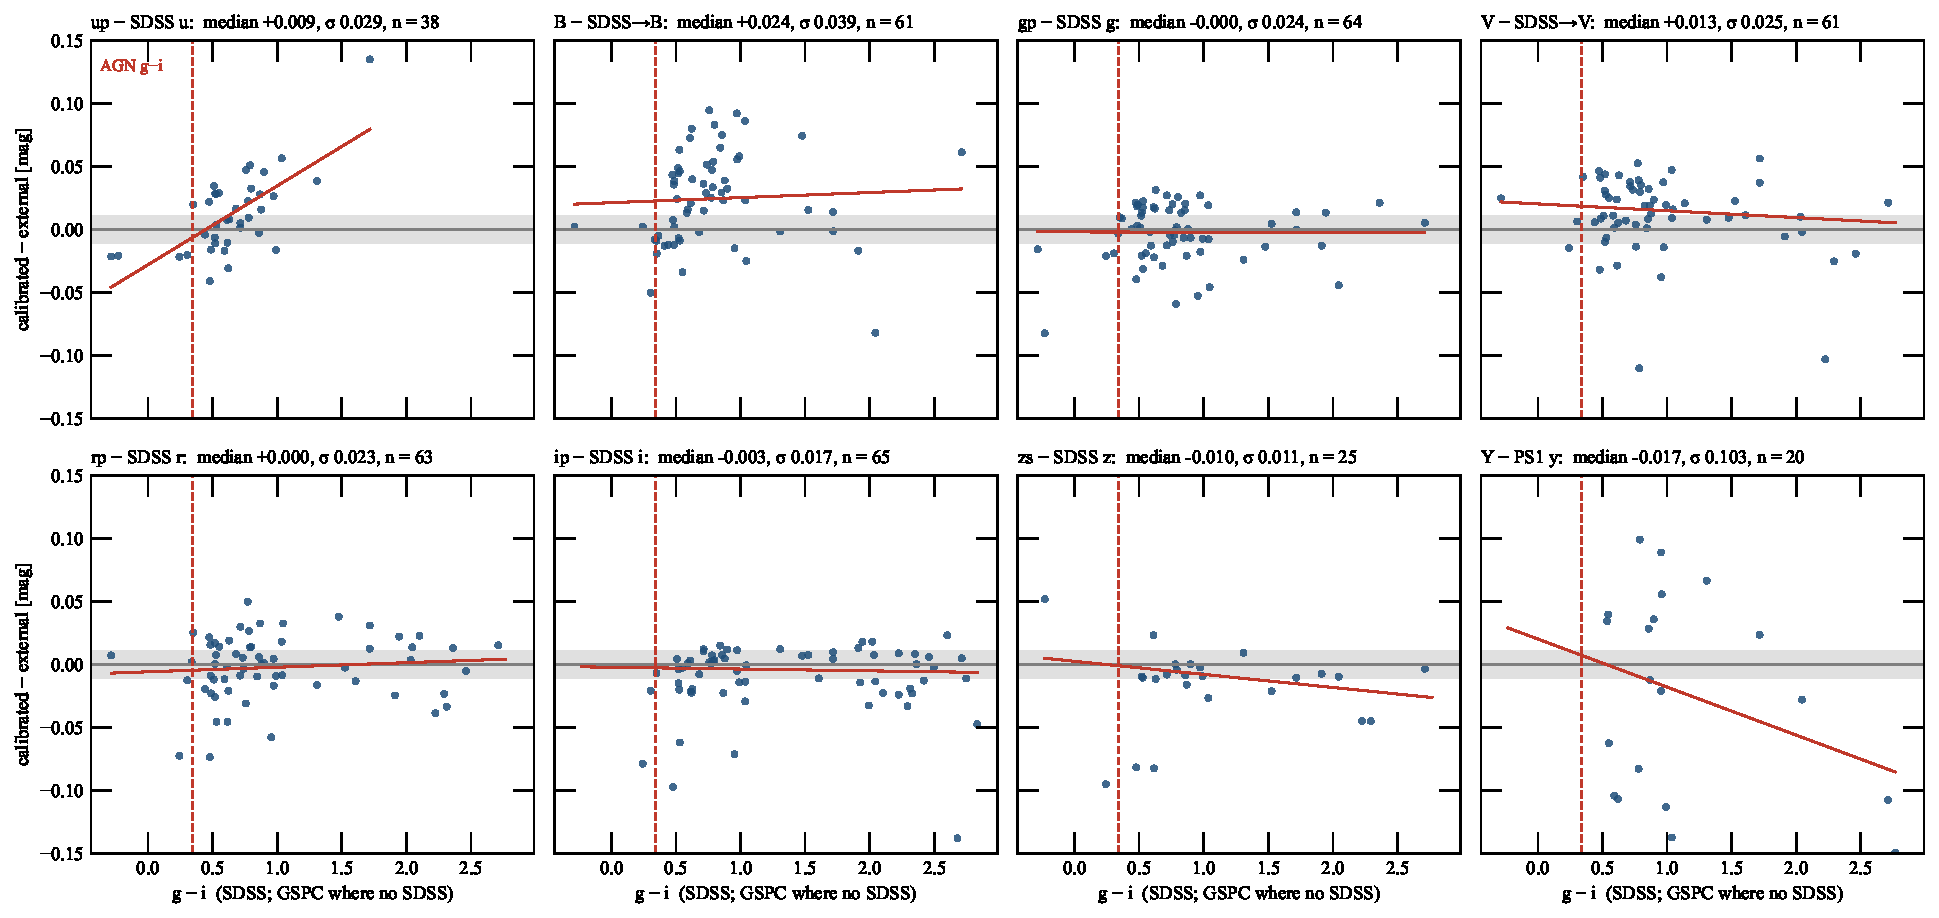
\includegraphics[width=\textwidth]{figures/abscal/abscal_01_stars.pdf}
  \caption{Mrk 817: PyTICS-calibrated comparison stars minus SDSS DR16 ($B$, $V$ via
  Jordi et al.\ 2006) and PS1 DR2 $y$, against $g-i$. Red line: clipped linear fit; dashed:
  AGN colour; grey band: $\pm0.01$\,mag.}
  \label{fig:mrk817-stars}
\end{figure}

\begin{figure}[htbp]
  \centering
  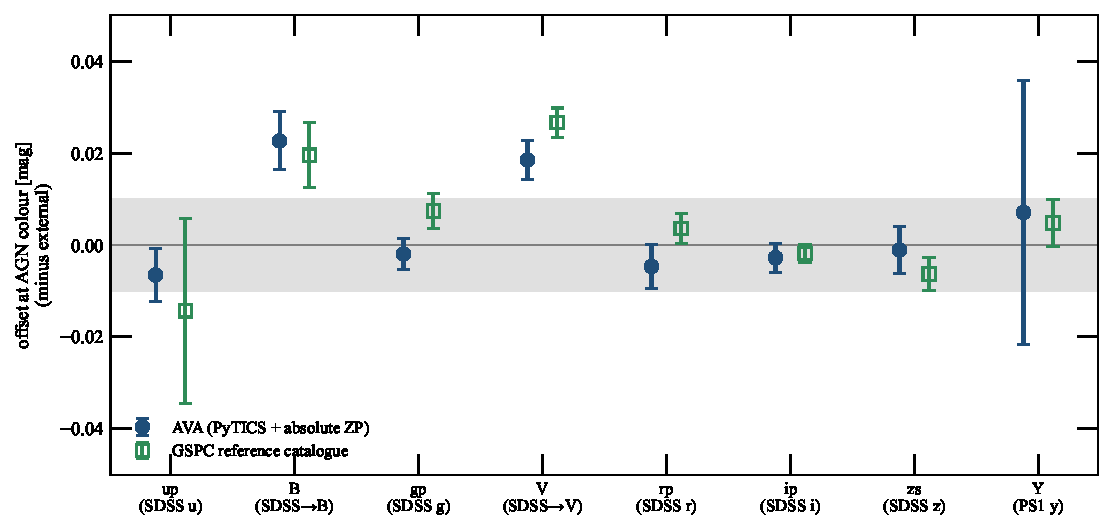
\includegraphics[width=0.75\textwidth]{figures/abscal/abscal_02_summary.pdf}
  \caption{Mrk 817: offset from the external photometry at the AGN colour, for the AVA
  calibration (filled) and for the GSPC reference catalogue (open).}
  \label{fig:mrk817-summary}
\end{figure}

\begin{figure}[htbp]
  \centering
  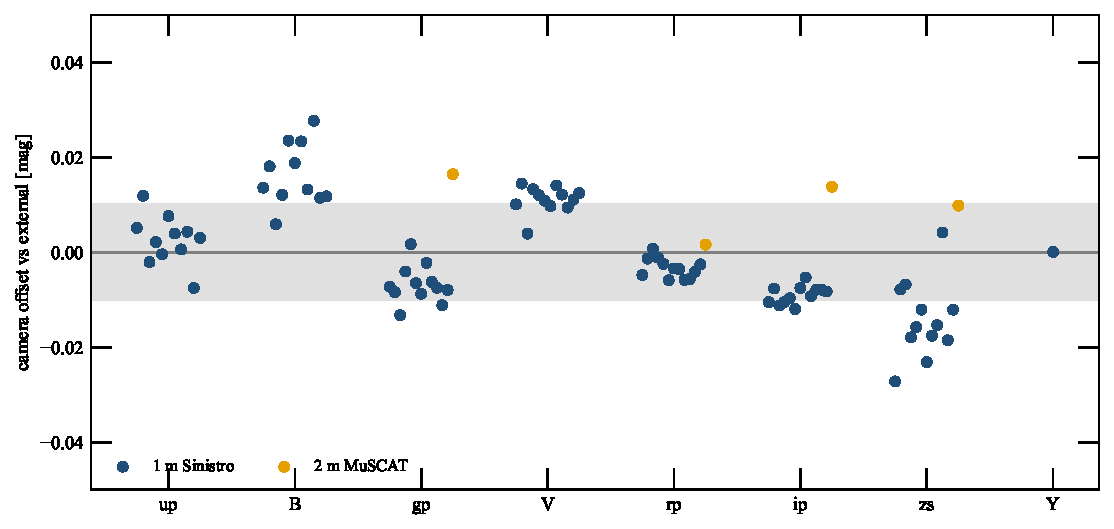
\includegraphics[width=0.75\textwidth]{figures/abscal/abscal_03_cameras.pdf}
  \caption{Mrk 817: per-camera offset from the external photometry (median over stars of
  each star's median calibrated magnitude in that camera).}
  \label{fig:mrk817-cameras}
\end{figure}

\begin{figure}[htbp]
  \centering
  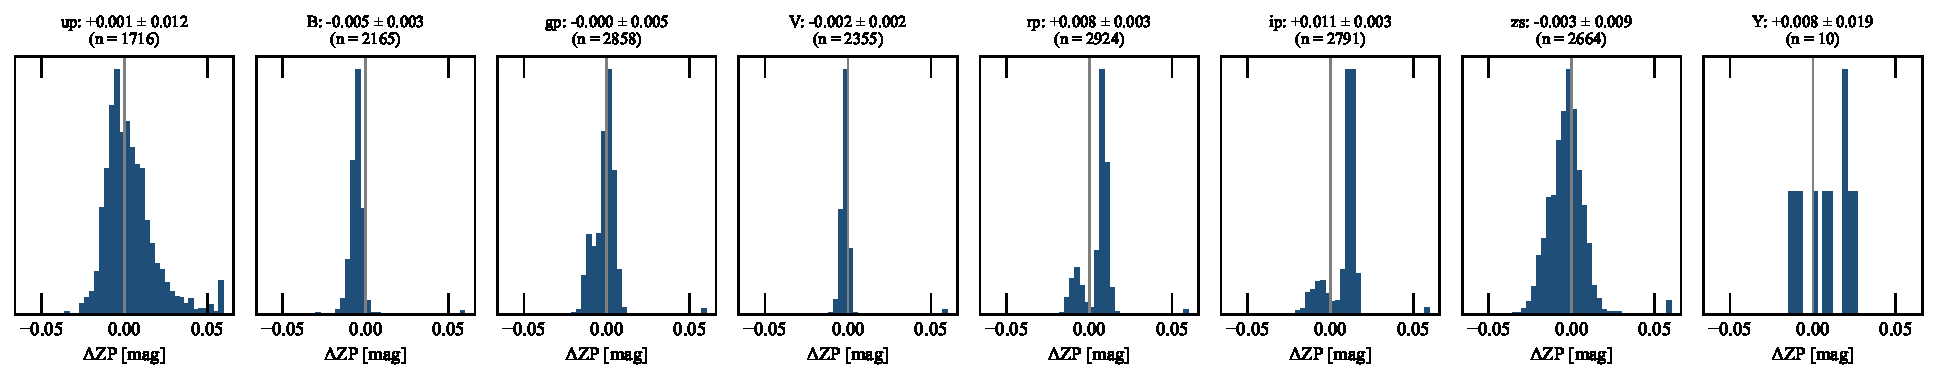
\includegraphics[width=\textwidth]{figures/abscal/abscal_04_frame_zp.pdf}
  \caption{Mrk 817: per-frame zero point from \texttt{frame\_qc} minus the ensemble
  zero point of the same frame (median $\pm$ robust $\sigma$). The secondary peak in $r$ and
  $i$ is MuSCAT (few ZP stars in its small field); Sinistro frames sit at a constant offset.
  The AGN light curve uses the ensemble zero point only.}
  \label{fig:mrk817-framezp}
\end{figure}

\begin{figure}[htbp]
  \centering
  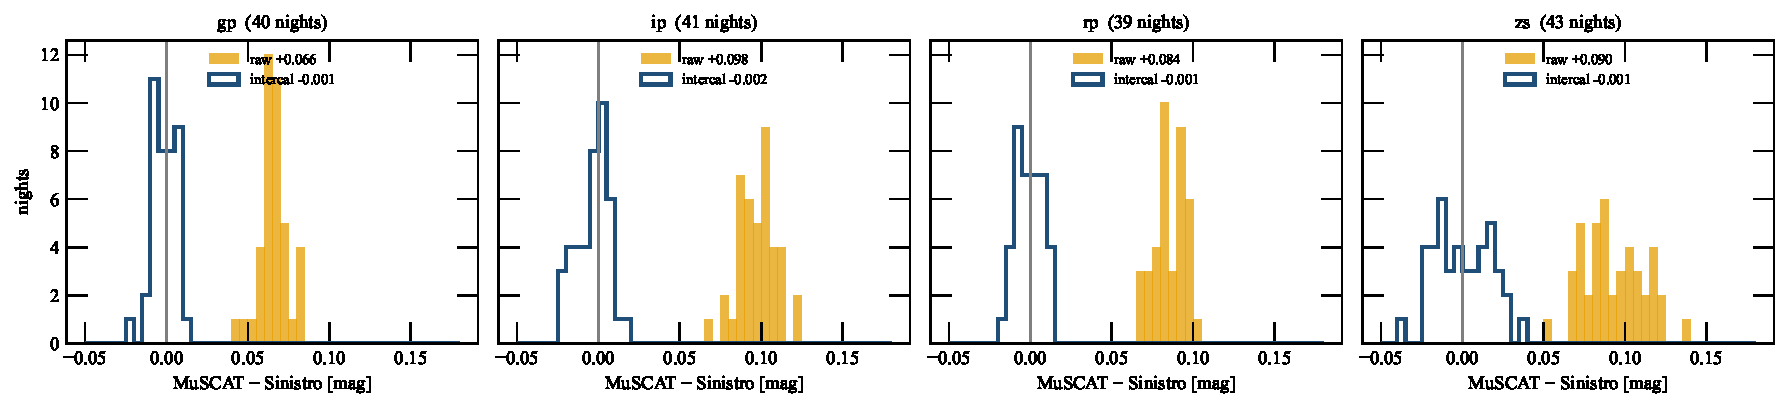
\includegraphics[width=\textwidth]{figures/abscal/abscal_05_muscat.pdf}
  \caption{Mrk 817: AGN, MuSCAT minus Sinistro on the same night, before (filled) and
  after (open) the additive intercal correction.}
  \label{fig:mrk817-muscat}
\end{figure}
 from docs/ (needs graphicx, booktabs).
\paragraph{Independent check of the absolute calibration (Mrk 817).}
The PyTICS-calibrated comparison stars were compared with photometry that AVA never
uses: SDSS DR16 PSF magnitudes ($u\,g\,r\,i\,z$; $B$, $V$ through the Jordi et al.\ 2006
stellar transformations, themselves good to $\sim$0.02--0.03\,mag) and Pan-STARRS1 DR2
$y$ (Table~\ref{tab:mrk817}, Figs.~\ref{fig:mrk817-stars}--\ref{fig:mrk817-summary}).
Evaluated at the AGN colour ($g-i=0.34$), $u\,g\,r\,i\,z$ agree with SDSS to
$\le0.007$\,mag and $B$, $V$ to $+0.019$--$+0.023$\,mag,
within the transformation uncertainty; the GSPC catalogue itself shows the same $B$, $V$
offset. Individual cameras agree to 0.002--0.010\,mag rms
(Fig.~\ref{fig:mrk817-cameras}), and the per-frame zero points of the \texttt{frame\_qc} path
agree with the ensemble to $\le0.011$\,mag (Fig.~\ref{fig:mrk817-framezp}).
MuSCAT measures the AGN $0.07$--$0.10$\,mag fainter than Sinistro on the same nights (8.9$''$ vs 10.5$''$ aperture: less host light); after the intercal correction the difference is $\le0.002$\,mag (Fig.~\ref{fig:mrk817-muscat}). $Y$ has only 10 epochs and a 0.10\,mag star-to-star scatter against PS1 and is not yet usable. The published fluxes use $f_\nu = 3631\,\mathrm{Jy}\times10^{-0.4\,m_{\rm AB}}$
(checked: ratio 0.99994). The comparison is limited by SDSS's own AB accuracy
($\sim$0.01--0.02\,mag, more in $u$) and tests point sources only; the AGN additionally
depends on the aperture host fraction and on emission lines within the filters.

\begin{table}[htbp]
  \centering\small
  \caption{Mrk 817: calibrated comparison stars minus external photometry (AB, mag).
  Median and robust $\sigma$ over stars; ``at AGN'' is a clipped linear fit in $g-i$ evaluated at
  the AGN colour (bootstrap error); GSPC is the reference catalogue against the same truth;
  camera rms is the scatter of per-camera offsets; ZP is the zero point applied to the AGN.}
  \label{tab:mrk817}
  \begin{tabular}{llrrrrrrr}
  \toprule
  Filter & External & $N$ & Median & $\sigma$ & At AGN & GSPC & Camera rms & ZP \\
  \midrule
  up & SDSS $u$ & 38 & $+0.009$ & 0.029 & $-0.007$\,$\pm$0.006 & $-0.014$ & 0.005 & 22.140 \\
  B & SDSS$\to B$ & 61 & $+0.024$ & 0.039 & $+0.023$\,$\pm$0.006 & $+0.020$ & 0.006 & 23.337 \\
  gp & SDSS $g$ & 64 & $-0.000$ & 0.024 & $-0.002$\,$\pm$0.003 & $+0.007$ & 0.007 & 23.926 \\
  V & SDSS$\to V$ & 61 & $+0.013$ & 0.025 & $+0.019$\,$\pm$0.004 & $+0.027$ & 0.003 & 23.412 \\
  rp & SDSS $r$ & 63 & $+0.000$ & 0.023 & $-0.005$\,$\pm$0.005 & $+0.004$ & 0.002 & 23.753 \\
  ip & SDSS $i$ & 65 & $-0.003$ & 0.017 & $-0.003$\,$\pm$0.003 & $-0.002$ & 0.006 & 23.328 \\
  zs & SDSS $z$ & 25 & $-0.010$ & 0.011 & $-0.001$\,$\pm$0.005 & $-0.006$ & 0.010 & 22.164 \\
  Y & PS1 $y$ & 20 & $-0.017$ & 0.103 & $+0.007$\,$\pm$0.029 & $+0.005$ & -- & 20.110 \\
  \bottomrule
  \end{tabular}
\end{table}

\begin{figure}[htbp]
  \centering
  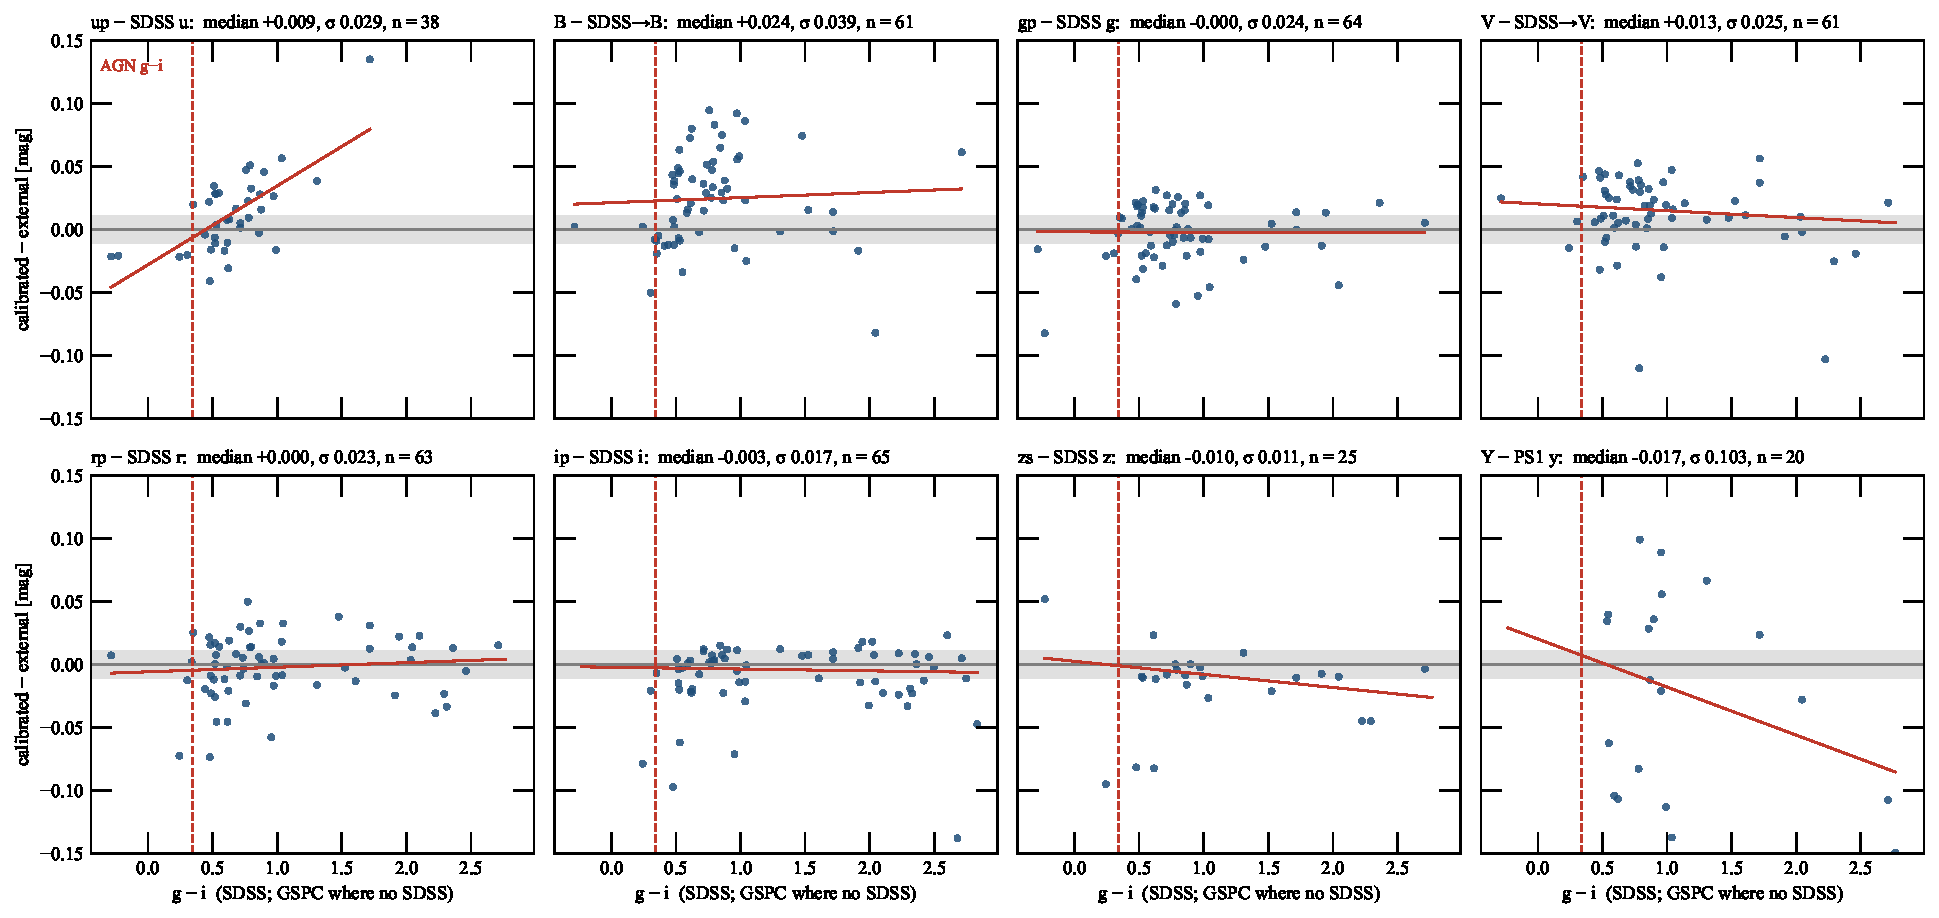
\includegraphics[width=\textwidth]{figures/abscal/abscal_01_stars.pdf}
  \caption{Mrk 817: PyTICS-calibrated comparison stars minus SDSS DR16 ($B$, $V$ via
  Jordi et al.\ 2006) and PS1 DR2 $y$, against $g-i$. Red line: clipped linear fit; dashed:
  AGN colour; grey band: $\pm0.01$\,mag.}
  \label{fig:mrk817-stars}
\end{figure}

\begin{figure}[htbp]
  \centering
  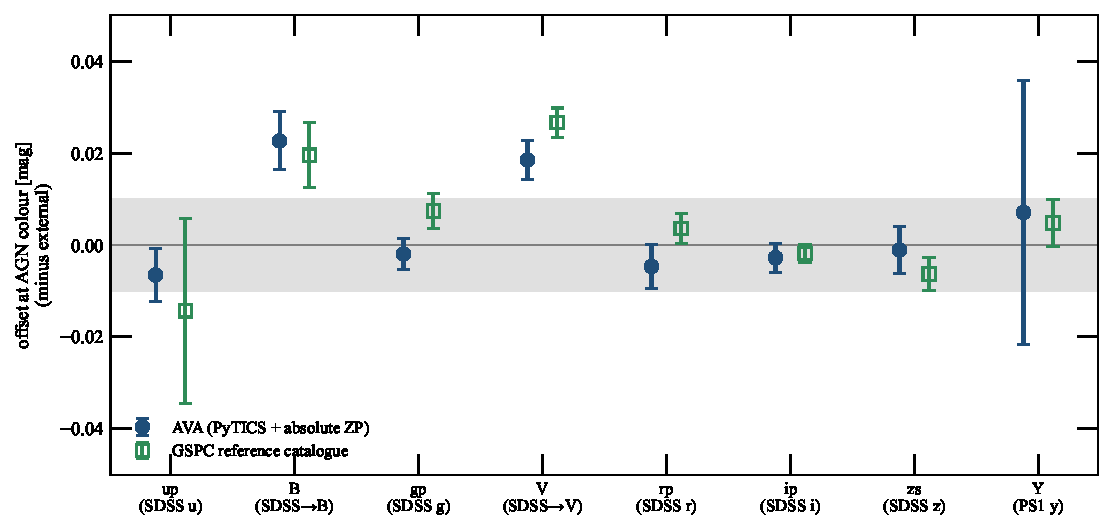
\includegraphics[width=0.75\textwidth]{figures/abscal/abscal_02_summary.pdf}
  \caption{Mrk 817: offset from the external photometry at the AGN colour, for the AVA
  calibration (filled) and for the GSPC reference catalogue (open).}
  \label{fig:mrk817-summary}
\end{figure}

\begin{figure}[htbp]
  \centering
  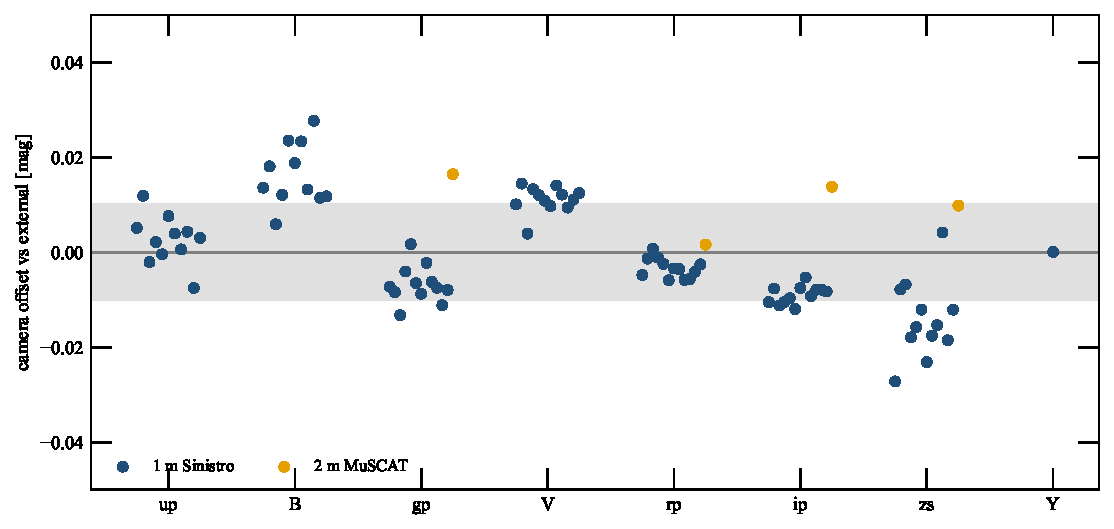
\includegraphics[width=0.75\textwidth]{figures/abscal/abscal_03_cameras.pdf}
  \caption{Mrk 817: per-camera offset from the external photometry (median over stars of
  each star's median calibrated magnitude in that camera).}
  \label{fig:mrk817-cameras}
\end{figure}

\begin{figure}[htbp]
  \centering
  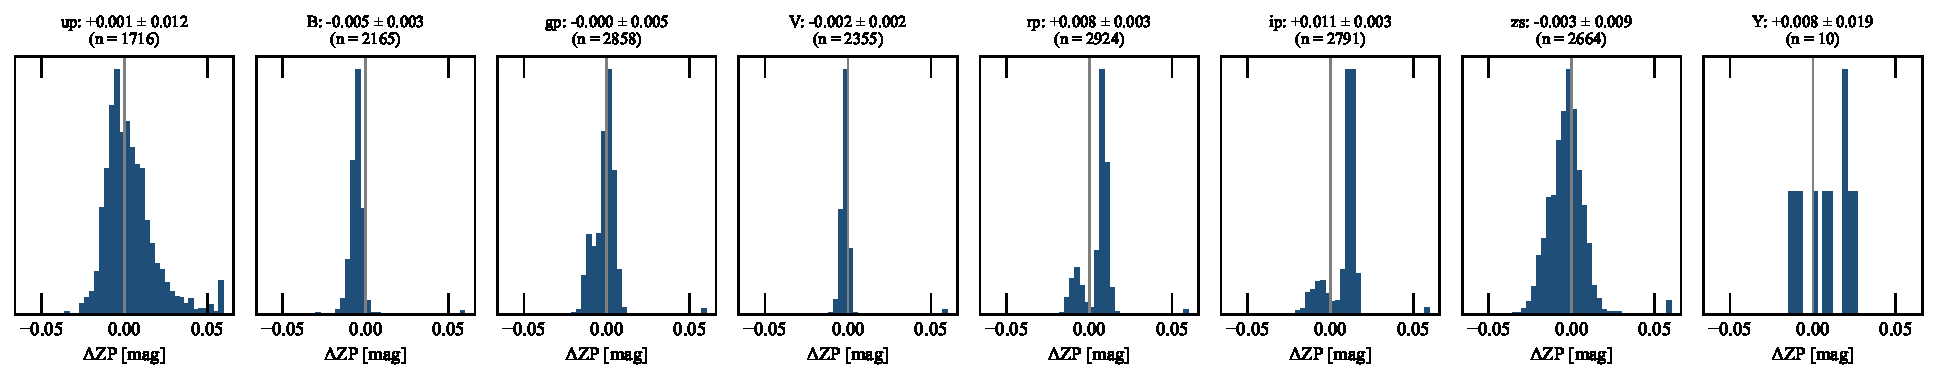
\includegraphics[width=\textwidth]{figures/abscal/abscal_04_frame_zp.pdf}
  \caption{Mrk 817: per-frame zero point from \texttt{frame\_qc} minus the ensemble
  zero point of the same frame (median $\pm$ robust $\sigma$). The secondary peak in $r$ and
  $i$ is MuSCAT (few ZP stars in its small field); Sinistro frames sit at a constant offset.
  The AGN light curve uses the ensemble zero point only.}
  \label{fig:mrk817-framezp}
\end{figure}

\begin{figure}[htbp]
  \centering
  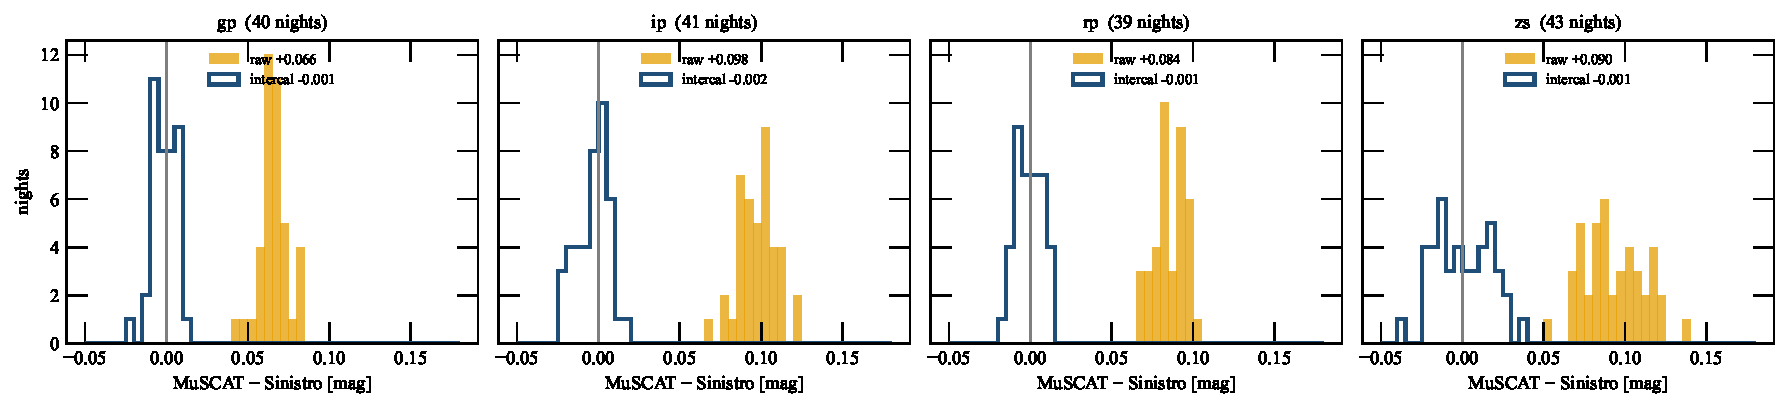
\includegraphics[width=\textwidth]{figures/abscal/abscal_05_muscat.pdf}
  \caption{Mrk 817: AGN, MuSCAT minus Sinistro on the same night, before (filled) and
  after (open) the additive intercal correction.}
  \label{fig:mrk817-muscat}
\end{figure}
